% In this file you should put the actual content of the blueprint.
% It will be used both by the web and the print version.
% It should *not* include the \begin{document}
%
% If you want to split the blueprint content into several files then
% the current file can be a simple sequence of \input. Otherwise It
% can start with a \section or \chapter for instance.

\chapter{Basic theory of magmas}

\begin{definition}[Magma]\label{magma-def}\lean{Magma}\leanok A \emph{magma} is a set $G$ equipped with a binary operation $\circ: G \times G \to G$.  A \emph{homomorphism} $\varphi : G \to H$ between two magmas is a map such that $\varphi(x \circ y) = \varphi(x) \circ \varphi(y)$ for all $x,y \in G$.  An \emph{isomorphism} is an invertible homomorphism.
\end{definition}

Groups, semi-groups, and monoids are familiar examples of magmas.  However, in general we do not expect magmas to have any associative properties.

A magma is called \emph{empty} if it has cardinality zero, \emph{singleton} if it has cardinality one, and \emph{non-trivial} otherwise.

The number of magma structures on a set $G$ of cardinality $n$ is of course $n^{n^2}$, which is \footnote{All sequences start from $n=0$ unless otherwise specified.}
$$ 1, 1, 16, 19683, 4294967296, 298023223876953125, \dots$$
(\href{OEIS A002489}{https://oeis.org/A002489}).
Up to isomorphism, the number of finite magmas of cardinality $n$ up to isomorphism is the slightly slower growing sequence
$$ 1, 1, 10, 3330, 178981952, 2483527537094825, 14325590003318891522275680, \dots$$
(\href{OEIS A001329}{https://oeis.org/A001329}).

\begin{definition}[Free Magma]\label{free-magma-def}\lean{FreeMagma}\leanok\uses{magma-def} The \emph{free magma} $M_X$ generated by a set $X$ (which we call an \emph{alphabet}) is the set of all finite formal expressions built from elements of $X$ and the operation $\circ$.  An element of $M_X$ will be called a \emph{word} with alphabet $X$.  The \emph{order} of a word is the number of $\circ$ symbols needed to generate the word.  Thus for instance $X$ is precisely the set of words of order $1$ in $M_X$.
\end{definition}

For sake of concreteness, we will take the alphabet $X$ to default to the natural numbers $\N$ if not otherwise specified.

For instance, if $X = \{0,1\}$, then $M_X$ would consist of the following words:
\begin{itemize}
  \item $0$, $1$ (the words of order $0$);
  \item $0 \circ 0$, $0 \circ 1$, $1 \circ 0$, $1 \circ 1$ (the words of order $1$);
  \item $0 \circ (0 \circ 0)$, $0 \circ (0 \circ 1)$, $0 \circ (1 \circ 0)$, $0 \circ (1 \circ 1)$, $1 \circ (0 \circ 0)$, $1 \circ (0 \circ 1)$, $1 \circ (1 \circ 0)$, $1 \circ (1 \circ 1)$, $(0 \circ 0) \circ 0$, $(0 \circ 0) \circ 1$, $(0 \circ 1) \circ 0$, $(0 \circ 1) \circ 1$, $(1 \circ 0) \circ 0$, $(1 \circ 0) \circ 1$, $(1 \circ 1) \circ 0$, $(1 \circ 1) \circ 1$ (the words of order $2$);
  \item etc.
\end{itemize}

\begin{lemma}  For a finite alphabet $X$, the number of words of order $n$ is $C_n |X|^{n+1}$, where $C_n$ is the $n^{\mathrm{th}}$ Catalan number and $X$ is the cardinality of $X$.
\end{lemma}

\begin{proof} Follows from standard properties of Catalan numbers.
\end{proof}

The first few Catalan numbers are
$$ 1, 1, 2, 5, 14, 42, 132, \dots$$
(\href{OEIS A000108}{https://oeis.org/A000108}).


\begin{definition}[Induced homomorphism]\label{induced-def}\uses{free-magma-def}  Given a function $f: X \to G$ from an alphabet $X$ to a magma $G$, the \emph{induced homomorphism} $\varphi_f: M_X \to G$ is the unique extension of $f$ to a magma homomorphism.  Similarly, if $\pi \colon X \to Y$ is a function, we write $\pi_* \colon M_X \to M_Y$ for the unique extension of $\pi$ to a magma homomorphism.
\end{definition}

For instance, if $f : \{0,1\} \to G$ maps $0,1$ to $x,y$ respectively, then
$$ \varphi_f(0 \circ 1) = x \circ y$$
$$ \varphi_f(1 \circ (0 \circ 1)) = y \circ (x \circ y)$$
and so forth.  If $\pi \colon \N \to \N$ is the map $\pi(n) := n+1$, then
$$ \pi_*(0 \circ 1) = 1 \circ 2$$
$$ \pi_*(1 \circ (0 \circ 1)) = 2 \circ (1 \circ 2)$$
and so forth.

\begin{definition}[Law]\label{law-def}\uses{induced-def}  Let $X$ be a set. A \emph{law} with alphabet $X$ is a formal expression of the form $w == w'$, where $w, w' \in M_X$ are words with alphabet $X$ (thus one can identify laws with alphabet $X$ with elements of $M_X \times M_X$).  A magma $G$ \emph{satisfies} the law $w == w'$ if we have $\varphi_f( w ) = \varphi_f ( w' )$ for all $f: X \to G$, in which case we write $G \models w == w'$.
\end{definition}

Thus, for instance, the commutative law
\begin{equation}\label{comm-law}
  0 \circ 1 == 1 \circ 0
\end{equation}
is satisfied by a magma $G$ if and only if
\begin{equation}\label{comm-law-2}
 x \circ y = y \circ x
\end{equation}
for all $x, y \in G$.  We refer to \eqref{comm-law-2} as the \emph{equation} associated to the law \eqref{comm-law}.  One can think of equations as the ``semantic'' intrepretation of a ``syntactic'' law.  However, we shall often abuse notation and a law with its associated equation thus we shall (somewhat carelessly) also refer to \eqref{comm-law-2} as ``the commutative law'' (rather than ``the commutative equation'').

\begin{lemma}[Pushforward]\label{push}\uses{law-def}  Let $w == w'$ be a law with some alphabet $X$, $G$ be a magma, and $\pi: X \to Y$ be a function.  If $G \models w == w'$, then $G \models \pi_*(w) == \pi_*(w')$.  In particular, if $\pi$ is a bijection, the statements If $G \models w == w'$, then $G \models \pi_*(w) == \pi_*(w')$ are equivalent.
\end{lemma}

If $\pi$ is a bijection, we will call $\pi_*(w) == \pi_*(w')$ a \emph{relabeling} of the law $w == w'$.  Thus for instance
$$ 5 \circ 7 == 7 \circ 5$$
is a relabeling of the commutative law \eqref{comm-law}.  By the above lemma, relabeling does not affect whether a given magna satisfies a given law.

\begin{proof}  Trivial.
\end{proof}

\begin{lemma}[Equivalence]\label{equiv}\uses{law-def}  Let $G$ be a magma and $X$ be an alphabet.  Then the relation $G \models w == w'$ is an equivalence relation on $M_X$.
\end{lemma}

\begin{proof}  Trivial.
\end{proof}

Define the total order of a law $w == w'$ to be the sum of the orders of $w$ and $w'$.

\begin{lemma}[Counting laws up to relabeling]\label{law-count}\uses{push}  Up to relabeling, the number of laws $w == w'$ of total order $n$ is $C_{n+1} B_{n+2}$.
\end{lemma}

\begin{proof} Follows from the properties of Catalan and Bell numbers.
\end{proof}

The first few Bell numbers (starting from $n=0$) are
$$ 1, 1, 2, 5, 15, 52, 203, \dots$$
(\href{OEIS A000110}{https://oeis.org/A000110}).

The sequence in Lemma \ref{law-count} is
$$ 2, 10, 75, 728, 8526, 115764, \dots$$
(\href{OEIS A289679}{https://oeis.org/A289679}).

Now we would also like to count laws up to relabeling and symmetry.

\begin{lemma}[Counting laws up to relabeling and symmetry]\label{law-count-sym}\uses{push} Up to relabeling and symmetry, the number of laws $w == w'$ of total order $n$ is
$$ C_{n+1} B_{n+2}/2$$
when $n$ is odd, and
$$ (C_{n+1} B_{n+2} + C_{n/2} (2D_{n+2} - B_{n+2}))/2$$
when $n$ is even, where $D_n$ is the number of partitions of $[n]$ up to reflection.
\end{lemma}

\begin{proof} Elementary counting.
\end{proof}

The sequence $D_n$ is (starting from $n=0$)
$$ 1, 1, 2, 4, 11, 32, 117, \dots$$
(\href{OEIS A103293}{https://oeis.org/A103293}), and the sequence in Lemma \ref{law-count-sym} is (starting from $n=0$)
$$ 2, 5, 41, 364, 4294, 57882, 888440, \dots$$
{\bf check this matches the formula}

We can also identify all laws of the form $w==w$ with the trivial law $0==0$.  The number of such laws of total order $n$ is zero if $n$ is odd, and $C_{n/2} B_{n/2+1}$ if $n$ is even.  We conclude:

\begin{lemma}[Counting laws up to relabeling, symmetry, and triviality]  Up to relabeling, symmetry, and triviality, the number of laws of total order $n$ is
$$ C_{n+1} B_{n+2}/2$$
if $n$ is odd, $2$ if $n = 0$, and
$$ (C_{n+1} B_{n+2} + C_{n/2} (2D_{n+2} - B_{n+2}))/2 - C_{n/2} B_{n/2+1}$$
if $n \geq 2$ is even.
\end{lemma}

\begin{proof} Routine counting.
\end{proof}

This sequence is
$$2, 5, 39, 364, 4284, 57882, 888365, \dots$$
{\bf check this matches the formula}.

In particular, up to relabeling, symmetry, and triviality, there are exactly $4694$ laws of total order at most $4$.  A list can be found \href{https://github.com/teorth/equational_theories/blob/main/data/equations.txt}{here}.  A script for generating them may be found \href{https://github.com/teorth/equational_theories/blob/main/scripts/generate_eqs_list.py}{here}.  The list is sorted by the total number of operations, then by the number of operations on the LHS. Within each such class we define an order on expressions by variable $<$ operation, and lexical order on variables.

\chapter{Subgraph laws}\label{subgraph-eq}

In this project we study the 4694 laws (up to symmetry and relabeling) of total order at most $4$.

Selected laws of interest are listed below, as well as in \href{https://github.com/teorth/equational_theories/blob/main/equational_theories/Equations.lean}{this file}.  Laws in this list will be referred to as ``subgraph equations'', as we shall inspect the subgraph of the implication subgraph induced by these equations.

\begin{definition}[Equation 1]\label{eq1}\lean{Equation1}\leanok\uses{magma-def}  Equation 1 is the law $0 \formaleq 0$ (or the equation $x=x$).
\end{definition}

This is the trivial law, satisfied by all magmas. It is self-dual.


\begin{definition}[Equation 2]\label{eq2}\lean{Equation2}\leanok\uses{magma-def}  Equation 2 is the law $0 \formaleq 1$ (or the equation $x=y$).
\end{definition}

This is the singleton law, satisfied only by the empty and singleton magmas.  It is self-dual.

\begin{definition}[Equation 3]\label{eq3}\lean{Equation3}\leanok\uses{magma-def}  Equation 3 is the law $0 \formaleq 0 \circ 0$ (or the equation $x = x \circ x$).
\end{definition}

This is the idempotence law.  It is self-dual.

\begin{definition}[Equation 4]\label{eq4}\lean{Equation4}\leanok\uses{magma-def}  Equation 4 is the law $0 \formaleq 0 \circ 1$ (or the equation $x = x \circ y$).
\end{definition}

This is the left absorption law.

\begin{definition}[Equation 5]\label{eq5}\lean{Equation5}\leanok\uses{magma-def}  Equation 5 is the law $0 \formaleq 1 \circ 0$ (or the equation $x = y \circ x$).
\end{definition}

This is the right absorption law (the dual of Definition \ref{eq4}).

\begin{definition}[Equation 6]\label{eq6}\lean{Equation6}\leanok\uses{magma-def}  Equation 6 is the law $0 \formaleq 1 \circ 1$ (or the equation $x = y \circ y$).
\end{definition}

This law is equivalent to the singleton law.

\begin{definition}[Equation 7]\label{eq7}\lean{Equation7}\leanok\uses{magma-def}  Equation 7 is the law $0 \formaleq 1 \circ 2$ (or the equation $x = y \circ z$).
\end{definition}

This law is equivalent to the singleton law.

\begin{definition}[Equation 8]\label{eq8}\lean{Equation8}\leanok\uses{magma-def}  Equation 8 is the law $0 \formaleq 0 \circ (0 \circ 0)$ (or the equation $x = x \circ (x \circ x)$).
\end{definition}

\begin{definition}[Equation 14]\label{eq14}\lean{Equation14}\leanok\uses{magma-def}  Equation 14 is the law $0 \formaleq  1 \circ (0 \circ 1)$ (or the equation $x = y ∘ (x ∘ y))$.
\end{definition}

Appears in Problem A1 from Putnam 2001.


\begin{definition}[Equation 23]\label{eq23}\lean{Equation23}\leanok\uses{magma-def}  Equation 23 is the law $0 \formaleq  (0 \circ 0) \circ 0$ (or the equation $x = (x \circ x) \circ x$).
\end{definition}

This is the dual of Definition \ref{eq8}.

\begin{definition}[Equation 29]\label{eq29}\lean{Equation29}\leanok\uses{magma-def}  Equation 29 is the law $0 \formaleq  (1 \circ 0) \circ 1$ (or the equation $x = (y ∘ x) ∘ y)$.
\end{definition}

Appears in Problem A1 from Putnam 2001.  Dual to Definition \ref{eq14}.

\begin{definition}[Equation 38]\label{eq38}\lean{Equation38}\leanok\uses{magma-def}  Equation 38 is the law $0 \circ 0  \formaleq  0 \circ 1$ (or the equation $x \circ x = x \circ y$).
\end{definition}

This law asserts that the magma operation is independent of the second argument.

\begin{definition}[Equation 39]\label{eq39}\lean{Equation39}\leanok\uses{magma-def}  Equation 39 is the law $0 \circ 0  \formaleq  1 \circ 0$ (or the equation $x \circ x = y \circ x$).
\end{definition}

This law asserts that the magma operation is independent of the first argument (the dual of Definition \ref{eq38}).

\begin{definition}[Equation 40]\label{eq40}\lean{Equation40}\leanok\uses{magma-def}  Equation 40 is the law $0 \circ 0  \formaleq  1 \circ 1$ (or the equation $x \circ x = y \circ y$).
\end{definition}

This law asserts that all squares are constant. It is self-dual.

\begin{definition}[Equation 41]\label{eq41}\lean{Equation41}\leanok\uses{magma-def}  Equation 41 is the law $0 \circ 0  \formaleq  1 \circ 2$ (or the equation $x \circ x = y \circ z$).
\end{definition}

This law is equivalent to the constant law, Definition \ref{eq46}.

\begin{definition}[Equation 42]\label{eq42}\lean{Equation42}\leanok\uses{magma-def}  Equation 42 is the law $0 \circ 1  \formaleq  0 \circ 2$ (or the equation $x \circ y = x \circ z$).
\end{definition}

Equivalent to Definition \ref{eq38}.

\begin{definition}[Equation 43]\label{eq43}\lean{Equation43}\leanok\uses{magma-def}  Equation 43 is the law $0 \circ 1  \formaleq  1 \circ 0$ (or the equation $x \circ y = y \circ x$).
\end{definition}

The commutative law. It is self-dual.

\begin{definition}[Equation 45]\label{eq45}\lean{Equation45}\leanok\uses{magma-def}  Equation 45 is the law $0 \circ 1  \formaleq  2 \circ 1$ (or the equation $x \circ y = z \circ y$).
\end{definition}

This is the dual of Definition \ref{eq42}.

\begin{definition}[Equation 46]\label{eq46}\lean{Equation46}\leanok\uses{magma-def}  Equation 46 is the law $0 \circ 1  \formaleq  2 \circ 3$ (or the equation $x \circ y = z \circ w$).
\end{definition}

The constant law: all products are constant. It is self-dual.

\begin{definition}[Equation 168]\label{eq168}\lean{Equation168}\leanok\uses{magma-def}  Equation 168 is the law $0  \formaleq  (1 \circ 0) \circ (0 \circ 2)$ (or the equation $x = (y \circ x) \circ (x \circ z)$).
\end{definition}

The law of a central groupoid. It is self-dual.

\begin{definition}[Equation 381]\label{eq381}\lean{Equation381}\leanok\uses{magma-def}  Equation 381 is the law $0 \circ 1  \formaleq  (0 \circ 2) \circ 1$ (or the equation $x \circ y = (x \circ z) \circ y$).
\end{definition}

Appears in Putnam 1978, Problem A4, part (b).

\begin{definition}[Equation 387]\label{eq387}\lean{Equation387}\leanok\uses{magma-def}  Equation 387 is the law $0 \circ 1  \formaleq  (1 \circ 1) \circ 0$ (or the equation $x \circ y = (y \circ y) \circ x$).
\end{definition}

\begin{definition}[Equation 3722]\label{eq3722}\lean{Equation3722}\leanok\uses{magma-def}  Equation 3722 is the law $0 \circ 1  \formaleq  (0 \circ 1) \circ (0 \circ 1)$ (or the equation $x \circ y = (x \circ y) \circ (x \circ y)$).
\end{definition}

Appears in Putnam 1978, Problem A4, part (a).  It is self-dual.

\begin{definition}[Equation 3744]\label{eq3744}\lean{Equation3744}\leanok\uses{magma-def}  Equation 3744 is the law $0 \circ 1  \formaleq  (0 \circ 2) \circ (3 \circ 1)$ (or the equation $x \circ y = (x \circ z) \circ (w \circ y)$).
\end{definition}

This law is called a ``bypass operation'' in Putnam 1978, Problem A4. It is self-dual.

\begin{definition}[Equation 4512]\label{eq4512}\lean{Equation4512}\leanok\uses{magma-def}  Equation 4512 is the law $0 \circ (1 \circ 2)  \formaleq  (0 \circ 1) \circ 2$ (or the equation $x \circ (y \circ z) = (x \circ y) \circ z$).
\end{definition}

The associative law. It is self-dual.

\begin{definition}[Equation 4513]\label{eq4513}\lean{Equation4513}\leanok\uses{magma-def}  Equation 4513 is the law $0 \circ (1 \circ 2)  \formaleq  (0 \circ 1) \circ 3$ (or the equation $x \circ (y \circ z) = (x \circ y) \circ w$).
\end{definition}

\begin{definition}[Equation 4522]\label{eq4522}\lean{Equation4522}\leanok\uses{magma-def}  Equation 4522 is the law $0 \circ (1 \circ 2)  \formaleq  (0 \circ 3) \circ 4$ (or the equation $x \circ (y \circ z) = (x \circ w) \circ u$).
\end{definition}

Dual to Definition \ref{eq4579}.

\begin{definition}[Equation 4564]\label{eq4564}\lean{Equation4564}\leanok\uses{magma-def}  Equation 4564 is the law $0 \circ (1 \circ 2)  \formaleq  (3 \circ 1) \circ 2$ (or the equation $x \circ (y \circ z) = (w \circ y) \circ z$).
\end{definition}

Dual to Definition \ref{eq4513}.

\begin{definition}[Equation 4579]\label{eq4579}\lean{Equation4579}\leanok\uses{magma-def}  Equation 4579 is the law $0 \circ (1 \circ 2)  \formaleq  (3 \circ 4) \circ 2$ (or the equation $x \circ (y \circ z) = (w \circ u) \circ z$).
\end{definition}

Dual to Definition \ref{eq4522}.

\begin{definition}[Equation 4582]\label{eq4582}\lean{Equation4582}\leanok\uses{magma-def}  Equation 4582 is the law $0 \circ (1 \circ 2)  \formaleq  (3 \circ 4) \circ 5$ (or the equation $x \circ (y \circ z) = (w \circ u) \circ v$).
\end{definition}

This law asserts that all triple constants (regardless of bracketing) are constant.

Here is a more complicated law, introduced by Kisielewicz \cite{Kisielewicz}:

\begin{definition}[Equation 374794]
  \lean{EquationKis}\leanok
  \label{eq374794}\uses{magma-def}
  Equation 374794 is the law $0  \formaleq  (((1 \circ 1) \circ 1) \circ 0) \circ ((1 \circ 1) \circ 2)$ (or the equation $x = (((y \circ y) \circ y) \circ x) \circ ((y \circ y) \circ z)$).
\end{definition}

We will be interested in seeing which laws imply which other laws, in the sense that magmas obeying the former law automatically obey the latter.  We will also be interested in \emph{anti-implications} showing that one law does \emph{not} imply another, by producing examples of magmas that obey the former law but not the latter.

The singleton or empty magma obeys all equational laws.  One can ask whether an equational law admits nontrivial finite or infinite models.  An \emph{Austin law} is a law which admits infinite models, but no nontrivial finite models.  Austin \cite{austin} established the first such law, namely the order $9$ law
$$ (((1 \circ 1) \circ 1) \circ 0) \circ (((1 \circ 1) \circ ((1 \circ 1) \circ 1)) \circ 2) = 0.$$
A shorter Austin law (order $6$) was established in \cite{Kisielewicz}:

\begin{theorem}[Kisielewicz theorem]
  \lean{InfModel.Finite.EquationKis_implies_Equation2,InfModel.EquationKis_not_implies_Equation2}\leanok
  \label{kis-thm}\uses{eq374794,eq2}
  Definition \ref{eq374794} is an Austin law.
\end{theorem}

\begin{proof} \leanok Suppose for contradiction that we have a non-trivial model of Definition \ref{eq374794}. Write $y^2 := y \circ y$ and $y^3 := y^2 \circ y$. For any $y,z$, introduce the functions $f_y: x \mapsto y^3 \circ x$ and $g_{yz}: x \mapsto x \circ (y^2 \circ z)$.  Definition \ref{eq374794} says that $g_{yz}$ is a left-inverse of $f_y$, hence by finiteness these are inverses and $g_{yz}$ is independent of $z$. In particular
$$ f(y^3) = g_{yy}(y^3) = g_{yz}(y^3) = f(y^2 \circ z)$$
and hence $y^2 \circ z$ is independent of $z$.  Thus
$$ f_y(x) = (y^2 \circ y) \circ x = (y^2 \circ y^2) \circ x$$
is independent of $x$.  As $f_y$ is invertible, this forces the magma to be trivial, a contradiction.

To construct an infinite magma, take the positive integers $\Z^+$ with the operation $x \circ y$ defined as
\begin{itemize}
  \item $2^x$ if $y=x$;
  \item $3^y$ if $x = 1 \neq y$;
  \item $\min(j,1)$ if $x=3^j$ and $y \neq x$; and
  \item $1$ otherwise.
\end{itemize}
Then $y^2 = 2^y$, $y^3 = 1$, and $y^2 \circ z$ a power of two for all $y, z$, and $(1 \circ x) \circ w = x$ for all $x$ whenever $w$ is a power of two, so Definition \ref{eq374794} is satisfied.
\end{proof}

An even shorter law (order $5$) was obtained by the same author in a followup paper \cite{Kisielewicz2}:

\begin{theorem}[Kisielewicz theoremII]\label{kis-thm2}\uses{eq2}
$(((1 \circ 1) \circ 1) \circ 0) \circ (1 \circ 2) \formaleq 0$ is an Austin law.
\end{theorem}

\begin{proof} Using the $y^2$ and $y^3$ notation as before, the law reads
\begin{equation}\label{kis2-law}
   (y^3 \circ x) \circ (y \circ z) = x.
  \end{equation}
In particular, for any $y$, the map $T_y \colon x \mapsto y^3 \circ x$ is injective, hence bijective in a finite model $G$.  In particular we can find a function $f : G \to G$ such that $T_y f(y) = y^3$ for all $y$  Applying \eqref{kis2-law} with $x = f(y)$, we conclude
$$ T_y(y \circ z) = y^3 \circ (y \circ z) = f(y) $$
and thus $y \circ z$ is independent of $z$ by injectivity of $T_y$.  Thus, the left-hand side of \eqref{kis2-law} does not depend on $x$, and so the model is trivial.  This shows there are no non-trivial finite models.

To establish an infinite model, use $\N$ with $x \circ y$ defined by requiring
$$ y \circ y = 2^y; \quad 2^y \circ y = 3^y$$
and
$$ 3^y \circ x = 3^y 5^x$$
for $x \neq 3^y$, and
$$ (3^y 5^x) \circ z = x$$
for $z \neq 3^y 5^x$.  Finally set
$$ 2^{3^y} \circ z = 3^y$$
for $z \neq 3^y, 2^{3^y}$.  All other assignments of $\circ$ may be made arbitrarily. It is then a routine matter to establish \eqref{kis2-law}.
\end{proof}

In that paper a computer search was also used to show that no law of order four or less is an Austin law.

\chapter{General implications}

\begin{definition}[Implication]\label{impl}\uses{law-def}  A law $w == w'$ is said to \emph{imply} another law $w'' == w'''$, if every magma $G$ that satisfies the former, satisfies the latter:
  $$ G \models w == w' \implies G \models w'' == w'''.$$
Two laws are said to be \emph{equivalent} if they imply each other.
\end{definition}

\begin{lemma}[Pre-order]\label{pre-order}\uses{impl}  Implication is a pre-order on the set of laws, and equivalence is an equivalence relation.
\end{lemma}

\begin{proof} Trivial.
\end{proof}

Implications between these laws are depicted in Figure \ref{fig:implications}.

\begin{figure}
  \centering
  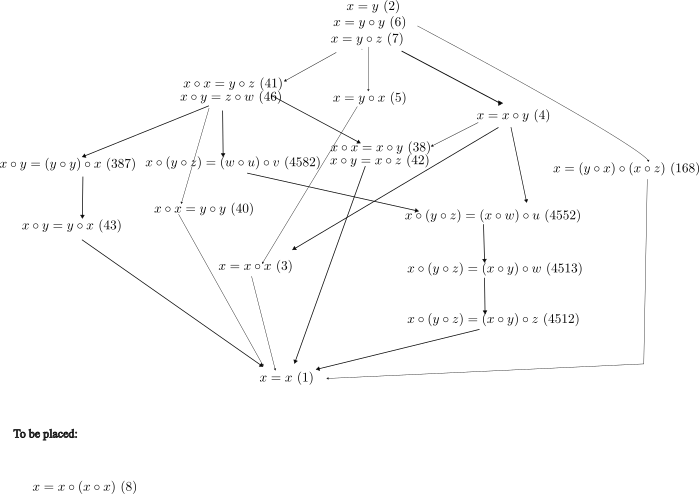
\includegraphics[width=0.5\linewidth]{../../images/implications.png}
  \caption{Implications between the above equations, displayed as a Hasse diagram.}
  \label{fig:implications}
\end{figure}


\begin{lemma}[Minimal element]\label{minimal}\uses{pre-order}  The law $0 == 0$ is the minimal element in this pre-order.
\end{lemma}

\begin{proof} Trivial.
\end{proof}

\begin{lemma}[Maximal element]\label{maximal}\uses{pre-order}  The law $0 == 0$ is the minimal element in this pre-order.
\end{lemma}

\begin{proof} Trivial.
\end{proof}

Every magma $G$ has a \emph{reversal} $G^{\mathrm{op}}$, formed by by replacing the magma operation $\circ$ with its opposite $\circ^{\mathrm{op}}:(x,y) \mapsto y \circ x$. There is a natural isomorphism between these magmas, which induces an involution $w \mapsto w^{\mathrm{op}}$ on words $w \in M_X$.  Every law $w == w'$ then has a \emph{dual} $w^{\mathrm{op}} == (w')^{\mathrm{op}}$.

For instance, the dual of the law $0 \circ 1 = 0 \circ 2$ is $1 \circ 0 = 2 \circ 0$, which after relabeling is $0 \circ 1 = 2 \circ 1$.  A list of equations and their duals can be found \href{https://github.com/teorth/equational_theories/blob/main/data/dual_equations.md}{here}.  Of the 4694 equations under consideration, 84 are self-dual, leaving 2305 pairs of dual equations.

The pre-ordering on laws has a duality symmetry:

\begin{lemma}[Duality of laws]\label{duality}\uses{pre-order}  If $w == w'$ implies $w'' == w'''$, then $w^{\mathrm{op}} == (w')^{\mathrm{op}}$ implies $w''^{\mathrm{op}} == (w''')^{\mathrm{op}}$.
\end{lemma}

\begin{proof} This follows from the fact that a magma $G$ satisfies a law $w == w'$ if and only if $G^{\mathrm{op}}$ satisfies $w^{\mathrm{op}} == (w')^{\mathrm{op}}$.
\end{proof}

Some equational laws can be ``diagonalized'':

\begin{theorem}[Diagonalization]\label{diag}  An equational law of the form
  \begin{equation}\label{prediag} F(x_1,\dots,x_n) = G(y_1,\dots,y_m),
  \end{equation}
  where $x_1,\dots,x_n$ and $y_1,\dots,y_m$ are distinct elements of the alphabet, implies the diagonalized law
$$ F(x_1,\dots,x_n) = F(x'_1,\dots,x'_n).$$
where $x'_1,\dots,x'_n$ are distinct from $x_1,\dots,x_n$
In particular, if $G(y_1,\dots,y_m)$ can be viewed as a specialization of $F(x'_1,\dots,x'_n)$, then these two laws are equivalent.
\end{theorem}

\begin{proof}  From two applications of \eqref{prediag} one has
$$ F(x_1,\dots,x_n) = G(y_1,\dots,y_m)$$
and
$$ F(x'_1,\dots,x'_n) = G(y_1,\dots,y_m)$$
whence the claim.
\end{proof}

Thus for instance, Definition \ref{eq7} is equivalent to Definition \ref{eq2}.

\chapter{Implications}

To reduce clutter, trivial or very easy implications will not be displayed here.

\begin{theorem}[387 implies 43]\label{387_implies_43}\uses{eq387,eq43}\lean{Subgraph.Equation387_implies_Equation43}\leanok  Definition \ref{eq387} implies Definition \ref{eq43}.
\end{theorem}

\begin{proof}\leanok (From \href{https://mathoverflow.net/a/450905/766}{MathOverflow}).
  By Definition \ref{eq387}, one has the law
\begin{equation}\label{387-again}
  (x \circ x) \circ y = y \circ x.
\end{equation}
Specializing to $y=x \circ x$, we conclude
$$(x \circ x) \circ (x \circ x) = (x \circ x) \circ x$$
and hence by another application of \eqref{eq387} we see that $x \circ x$ is idempotent:
\begin{equation}\label{idem}
  (x \circ x) \circ (x \circ x) = x \circ x.
\end{equation}
Now, replacing $x$ by $x \circ x$ in \eqref{387-again} and then using \eqref{idem} we see that
$$ (x \circ x) \circ y = y \circ (x \circ x)$$
so in particular $x \circ x$ commutes with $y \circ y$:
\begin{equation}\label{op-idem} (x \circ x) \circ (y \circ y) = (y \circ y) \circ (x \circ x).
\end{equation}
Also, from two applications of \eqref{387-again} one has
$$(x \circ x) \circ (y \circ y) = (y \circ y) \circ x = x \circ y.$$
Thus \eqref{op-idem} simplifies to $x \circ y = y \circ x$, which is Definition \ref{eq43}.
\end{proof}

\begin{theorem}[7 equivalent to 2]\label{7_equiv_2}\uses{eq2,eq7}\lean{Subgraph.Equation7_implies_Equation2, Subgraph.Equation2_implies_Equation7}\leanok  Definition \ref{eq7} is equivalent to Definition \ref{eq2}.
\end{theorem}

\begin{proof}\leanok
  When $x = y * z$, obviously $x = y$ because $x = x * x$ and $y = x * x$. the other way around is trivial.
\end{proof}

\begin{theorem}[6 equivalent to 2]\label{6_equiv_2}\uses{eq2,eq6}\lean{Subgraph.Equation6_implies_Equation2, Subgraph.Equation2_implies_Equation6}\leanok  Definition \ref{eq6} is equivalent to Definition \ref{eq2}.
\end{theorem}

\begin{proof}\leanok  Similar to the previous argument.
\end{proof}

More generally, any equation of the form $x = f(y,z,w,u,v)$ is equivalent to Equation 2 (eventually once we have enough API for Magma relations, we could formalize this general claim rather than establish it on a case by case basis).  It is also trivial that Equation 2 implies every other equation.

\chapter{Counterexamples}

\begin{theorem}[46 does not imply 4]\label{46_not_imply_4}\lean{Subgraph.Equation46_not_implies_Equation4}\leanok\uses{eq46,eq4} Definition \ref{eq46} does not imply Definition \ref{eq4}.
\end{theorem}

\begin{proof}\leanok Use the natural numbers $\N$ with operation $x \circ y := 0$.
\end{proof}

\begin{theorem}[4 does not imply 4582]\label{4_not_imply_4582}\lean{Subgraph.Equation4_not_implies_Equation4582}\leanok\uses{eq4,eq4582} Definition \ref{eq4} does not imply Definition \ref{eq4582}.
\end{theorem}

\begin{proof}\leanok Use the natural numbers $\N$ with operation $x \circ y := x$.
\end{proof}

\begin{theorem}[4 does not imply 43]\label{4_not_imply_43}\lean{Subgraph.Equation4_not_implies_Equation43}\leanok\uses{eq4,eq43} Definition \ref{eq4} does not imply Definition \ref{eq43}.
\end{theorem}

\begin{proof}\leanok Use the natural numbers $\N$ with operation $x \circ y := x$.
\end{proof}

\begin{theorem}[4582 does not imply 42]\label{4582_not_imply_42}\lean{Subgraph.Equation4582_not_implies_Equation42}\leanok\uses{eq4582,eq42} Definition \ref{eq4582} does not imply Definition \ref{eq42}.
\end{theorem}

\begin{proof}\leanok Use the natural numbers $\N$ with operation
$x \circ y$ equal to $1$ if $x=y=0$ and $2$ otherwise.
\end{proof}

\begin{theorem}[4582 does not imply 43]\label{4582_not_imply_43}\lean{Subgraph.Equation4582_not_implies_Equation43}\leanok\uses{eq4582,eq43} Definition \ref{eq4582} does not imply Definition \ref{eq43}.
\end{theorem}

\begin{proof}\leanok Use the natural numbers $\N$ with operation $x \circ y$ equal to $3$ if $x=1$ and $y=2$ and $4$ otherwise.
\end{proof}

\begin{theorem}[42 does not imply 43]\label{42_not_imply_43}\lean{Subgraph.Equation42_not_implies_Equation43}\leanok\uses{eq42,eq43} Definition \ref{eq42} does not imply Definition \ref{eq43}.
\end{theorem}

\begin{proof}\leanok Use the natural numbers $\N$ with operation $x \circ y := x$.
\end{proof}

\begin{theorem}[42 does not imply 4512]\label{42_not_imply_4512}\lean{Subgraph.Equation42_not_implies_Equation4512}\leanok\uses{eq42,eq4512} Definition \ref{eq42} does not imply Definition \ref{eq4512}.
\end{theorem}

\begin{proof}\leanok Use the natural numbers $\N$ with operation $x \circ y := x+1$.
\end{proof}

\begin{theorem}[43 does not imply 42]\label{43_not_imply_42}\lean{Subgraph.Equation43_not_implies_Equation42}\leanok\uses{eq43,eq42} Definition \ref{eq43} does not imply Definition \ref{eq42}.
\end{theorem}

\begin{proof}\leanok Use the natural numbers $\N$ with operation $x \circ y := x+y$.
\end{proof}

\begin{theorem}[43 does not imply 4512]\label{43_not_imply_4512}\lean{Subgraph.Equation43_not_implies_Equation4512}\leanok\uses{eq43,eq4512} Definition \ref{eq43} does not imply Definition \ref{eq4512}.
\end{theorem}

\begin{proof}\leanok Use the natural numbers $\N$ with operation $x \circ y := x \cdot y + 1$.
\end{proof}

\begin{theorem}[4513 does not imply 4522]\label{4513_not_imply_4522}\lean{Subgraph.Equation4513_not_implies_Equation4522}\leanok\uses{eq4513,eq4522} Definition \ref{eq4513} does not imply Definition \ref{eq4522}.
\end{theorem}

\begin{proof}\leanok Use the natural numbers $\N$ with operation $x \circ y$ equal to $1$ if $x=0$ and $y \leq 2$, $2$ if $x=0$ and $y>2$, and $x$ otherwise.
\end{proof}

\begin{theorem}[4512 does not imply 4513]\label{4512_not_imply_4513}\lean{Subgraph.Equation4512_not_implies_Equation4513}\leanok\uses{eq4512,eq4513} Definition \ref{eq4512} does not imply Definition \ref{eq4513}.
\end{theorem}

\begin{proof}\leanok Use the natural numbers $\N$ with operation $x \circ y := x + y$.
\end{proof}

\begin{theorem}[387 does not imply 42]\label{387_not_imply_42}\lean{Subgraph.Equation387_not_implies_Equation42}\leanok\uses{eq387,eq42} Definition \ref{eq387} does not imply Definition \ref{eq42}.
\end{theorem}

\begin{proof}\leanok Use the boolean type $\mathrm{Bool}$ with $x \circ y := x || y$.
\end{proof}

\begin{theorem}[43 does not imply 387]\label{43_not_imply_387}\lean{Subgraph.Equation43_not_implies_Equation387}\leanok\uses{eq43,eq387} Definition \ref{eq43} does not imply Definition \ref{eq387}.
\end{theorem}

\begin{proof}\leanok Use the natural numbers $\N$ with $x \circ y := x+y$.
\end{proof}

\begin{theorem}[387 does not imply 4512]\label{387_not_imply_4512}\lean{Subgraph.Equation387_not_implies_Equation4512}\leanok\uses{eq387,eq4512} Definition \ref{eq387} does not imply Definition \ref{eq4512}.
\end{theorem}

\begin{proof}\leanok Use the reals $\R$ with $x \circ y := (x+y)/2$.
\end{proof}

\begin{theorem}[3 does not imply 42]\label{3_not_imply_42}\lean{Subgraph.Equation3_not_implies_Equation42}\leanok\uses{eq3,eq42} Definition \ref{eq3} does not imply Definition \ref{eq42}.
\end{theorem}

\begin{proof}\leanok Use the natural numbers $\N$ with $x \circ y := y$.
\end{proof}

\begin{theorem}[3 does not imply 4512]\label{3_not_imply_4512}\lean{Subgraph.Equation3_not_implies_Equation4512}\leanok\uses{eq3,eq4512} Definition \ref{eq3} does not imply Definition \ref{eq4512}.
\end{theorem}

\begin{proof}\leanok Use the natural numbers $\N$ with $x \circ y$ equal to $x$ when $x=y$ and $x+1$ otherwise.
\end{proof}

\begin{theorem}[46 does not imply 3]\label{46_not_imply_3}\lean{Subgraph.Equation46_not_implies_Equation3}\leanok\uses{eq46,eq3} Definition \ref{eq46} does not imply Definition \ref{eq3}.
\end{theorem}

\begin{proof}\leanok Use the natural numbers $\N$ with $x \circ y := 0$.
\end{proof}

\begin{theorem}[43 does not imply 3]\label{43_not_imply_3}\lean{Subgraph.Equation43_not_implies_Equation3}\leanok\uses{eq43,eq3} Definition \ref{eq43} does not imply Definition \ref{eq3}.
\end{theorem}

\begin{proof}\leanok Use the natural numbers $\N$ with $x \circ y := x+y$.
\end{proof}

\chapter{Equivalence with the constant and singleton laws}

\href{https://github.com/teorth/equational_theories/blob/main/equational_theories/Generated/Constant.lean}{85 laws} have been shown to be equivalent to the constant law (Definition \ref{eq46}), and \href{https://github.com/teorth/equational_theories/blob/main/equational_theories/Generated/Singleton.lean}{815 laws} have been shown to be equivalent to the singleton law (Definition \ref{eq2}).

These are the laws up to 4 operations that follow from diagonalization of \ref{eq2} and of \ref{eq46}.

In order to formalize these in Lean, a search was run on the list of equations to discover
diagonalizations of these two specific laws: equations of the form $x = R$ where $R$ doesn't include
$x$, and equations of the form $x \circ y = R$ where R doesn't include $x$ or $y$.

The proofs themselves all look alike, and correspond exactly to the two steps described in the proof
of \ref{diag}. The Lean proofs were generated semi-manually, using search-and-replace starting from
the output of \texttt{grep} that found the diagonalized laws.

In the case of the constant law, equation \ref{eq41} ($x \circ x = y \circ z$) wasn't detected using
this method. It was added manually to the file with the existing proof from the sub-graph project.

\chapter{Simple rewrites}

\href{https://github.com/teorth/equational_theories/tree/main/equational_theories/SimpleRewrites/theorems}{53,905 implications} were automatically generated by simple rewrites.

{\bf describe the process of automatically generating these implications here.}

\chapter{Trivial auto-generated theorems}

\href{https://github.com/teorth/equational_theories/tree/main/equational_theories/Generated/TrivialBruteforce/theorems}{4.2m implications proven by a transitive reduction of 15k theorems} were proven using simple rewrite proof scripts.

{\bf include more details of the methodology, and any comparisons with other generated implication data sets.}


\bibliographystyle{plain} % We choose the "plain" reference style
\bibliography{references}
